\documentclass{beamer}
% Font - Arev
\usepackage[T1]{fontenc}
\usepackage{arev}
%\renewcommand*\familydefault{\sfdefault} %% Only if the base font of the document is to be sans serif

% for themes, etc.
%\mode<presentation>
%{ \usetheme{boxes} }

% Standard header

\usepackage{graphicx}
\usepackage{amsmath}   
\usepackage{amsthm}     
\usepackage[retainorgcmds]{IEEEtrantools}
\usepackage{xcolor}
\usepackage{thumbpdf}
\usepackage{multicol}   
\usepackage{graphicx}   
\usepackage{listings}
\usepackage{algorithm}
\usepackage{algorithmic}

\usepackage{hyperref}
\hypersetup{ 
  pdftitle          = {Learning in a Small World},
  pdfsubject        = {Learning in a Small World},
  pdfauthor         = {Arun Tejasvi Chaganty <arunchaganty@gmail.com>},
  pdfkeywords       = {},
  pdfcreator        = {pdflatex},
  pdfproducer       = {LaTeX with hyperref and thumbpdf},
  pdfstartpage      = {1},
  pdfpagemode       = UseThumbs,
  colorlinks        = true,
  linkcolor         = red,
  anchorcolor       = red,
  citecolor         = blue,
  filecolor         = red,
  urlcolor          = red
}

% Section References
\newcommand{\secref}[1] {\hyperref[#1]{Section~\ref*{#1}}}
\newcommand{\eqnref}[1] {Equation \eqref{#1}}
\newcommand{\thmref}[1] {Theorem \ref{#1}}
\newcommand{\lmref}[1] {Lemma \ref{#1}}
\newcommand{\algoref}[1] {\hyperref[#1]{Algorithm~\ref*{#1}}}
%\renewcommand{\algorithmiccomment}[1]{\textit{// #1}}
%\theoremstyle{plain} \newtheorem{thm}{Theorem}

%Math Operators
\DeclareMathOperator {\argmax} {argmax}
\DeclareMathOperator {\sgn} {sgn}
\DeclareMathOperator {\trace} {tr}
\DeclareMathOperator{\E} {E}
\DeclareMathOperator{\Var} {Var}

\renewcommand{\Re} {\mathbb{R}}

\newcommand{\ud}{\, \mathrm{d}}
\newcommand{\diff}[1] {\frac{\partial}{\, \partial #1}}
\newcommand{\diffn}[2] {\frac{\partial^{#2}}{\, \partial {#1}^{#2}}}
\newcommand{\tuple}[1] {\langle #1 \rangle}

%Short hand
\newcommand{\mdp} {\ensuremath{\mathcal{M}}}
\newcommand{\states} {\mathcal{S}}
\newcommand{\actions} {\mathcal{A}}
\newcommand{\transitions} {\mathcal{P}}
\newcommand{\rewards} {\mathcal{R}}
\newcommand{\graph} {\mathcal{G}}
\newcommand{\policy} {\pi}
\newcommand{\initset} {\mathcal{I}}
\newcommand{\stopcond} {\beta}
\newcommand{\option} {\tuple{ \initset,\policy,\stopcond} }
\newcommand{\options} {\mathcal{O}}

%Math Operators
\DeclareMathOperator {\ball} {B}
\DeclareMathOperator {\ballf} {B^{f}}
\DeclareMathOperator {\sball} {b}
\DeclareMathOperator {\sballf} {b^{f}}

%Short hand
\newcommand{\arbcnst} {\tilde{c}}
\newcommand{\greedyalgo} {\ensuremath{\mathcal{GA}~}}


% these will be used later in the title page
\title{Learning in a Small World}
\author{Arun Tejasvi Chaganty\\ Prateek Gaur}

% have this if you'd like a recurring outline
\AtBeginSection[]  % "Beamer, do the following at the start of every section"
{
\begin{frame}<beamer> 
\frametitle{Outline} % make a frame titled "Outline"
\tableofcontents[currentsection]  % show TOC and highlight current section
\end{frame}
}

\begin{document}

% this prints title, author etc. info from above
\begin{frame}
\titlepage
\end{frame}

\begin{frame}
\frametitle{Outline} % make a frame titled "Outline"
\tableofcontents  % show TOC and highlight current section
\end{frame}

\section{Motivation}
\label{sec:motivation}

\begin{frame}
    \frametitle{Motivation}
    \label{frame:motivation}
    
    \begin{itemize}
            \item How do we put together that which we have already learnt to accomplish a {\em new} task?
            \pause 
            \item Optimal solutions vs. composable solutions?
    \end{itemize}

\end{frame}

\section{Abstracting the Problem}
\label{sec:abstraction}

\begin{frame}
    \frametitle{Reinforcement Learning}
    \label{frame:abstraction-rl}

    \begin{figure}[h]
        \centering
        \includegraphics[width=3in]{figures/agent-environment}
        \label{fig:agent-environment}
        \caption{Agent-Environment Interface}
    \end{figure}

    \begin{itemize}
            \item An MDP $\mdp = \tuple{ \states, \actions, \transitions, \rewards }$
            \item Objective is to learn a policy $\pi : \states \to \actions$
            \item What action should an agent perform in a state to maximise
                reward.
            \item Typical approach: learn the `value' of a state.
    \end{itemize}
\end{frame}

\begin{frame}
    \frametitle{Subtasks: The Options Framework}
    \label{frame:abstraction-options}

    \begin{itemize}
        \item An `option' $\tuple{ \initset, \policy, \stopcond }$ is an extended action.
        \item Select the option in any state $s \in \initset$, and follow $\pi$
            till you reach a state $s'$ such that $\stopcond(s')$ is true.
    \end{itemize}
    % Paths in the state space
\end{frame}

\begin{frame}
    \frametitle{Defining the Problem}
    \label{frame:abstraction-problem}
    % Statement of the high level theorem we wish to prove
    \begin{itemize}
        \item We desire an environment where an agent can reach a state of {\em
            maximal value} for a task using only local information.
            \pause
            \begin{itemize}
                \item By efficient we loosely aim for {\em logarithmic number of choices}.
            \end{itemize}
    \end{itemize}
\end{frame}

\section{Small Worlds}
\label{sec:small-worlds}

\begin{frame}
    \frametitle{The Phenomenon}
    \label{frame:small-worlds-phenomenon}

    \begin{itemize}
            \item Six degrees of separation
            \pause
            \item A network has the small world property if individuals can
                transmit a message to a destination efficiently using only the
                information of the location of their direct acquaintances.
    \end{itemize}

\end{frame}

\begin{frame}
    \frametitle{Model}
    \label{frame:small-worlds-decentralised}
     
    \begin{figure}[h]
        \centering
        \includegraphics[width=2in]{figures/sw}
        \label{fig:small-world}
        \caption{Links in a Small World}
    \end{figure}

    \begin{itemize}
            \item Nodes arranged in a $k$-dimensional lattice.
            \item Each node has one long-range link, distributed according to
                $P_{k}( u, v ) \propto \dist(u,v)^{-k}$.
            \pause 
            \item A greedy algorithm can be constructed whose expected delivery
                time is polynomial in shortest path length.
    \end{itemize}

\end{frame}

\section{Making Learning Small World}
\label{sec:swoptions}

\begin{frame}
    \frametitle{Generating Options}
    \label{frame:swoptions-options}
    \begin{itemize}
            \item The state space is our network - immediate neighbours
                connected by primitive actions.
            \item Non-neighbouring nodes are connected using options with an
                optimal policy; 
            \item The long-range link is also distributed according to
                $P_{r}( u, v ) \propto \dist(u,v)^{-r}$.
            \pause 
            \item What does dimension mean? (Heuristic: Use number of neighbours
                by 2)
    \end{itemize}

\end{frame}

\section{Results}

\begin{frame}
    \frametitle{Rooms}
    \label{frame:results-rooms-domain}
    % Paths in the state space
    \begin{figure}[h]
        \centering
        \includegraphics[width=2.5in]{figures/rooms-options}
        \label{fig:rooms-domain}
        \caption{Options Learnt in Rooms}
    \end{figure}
\end{frame}

\begin{frame}
    \frametitle{Rooms}
    \label{frame:results-rooms-results}
    % Paths in the state space
    \begin{figure}[h]
        \centering
        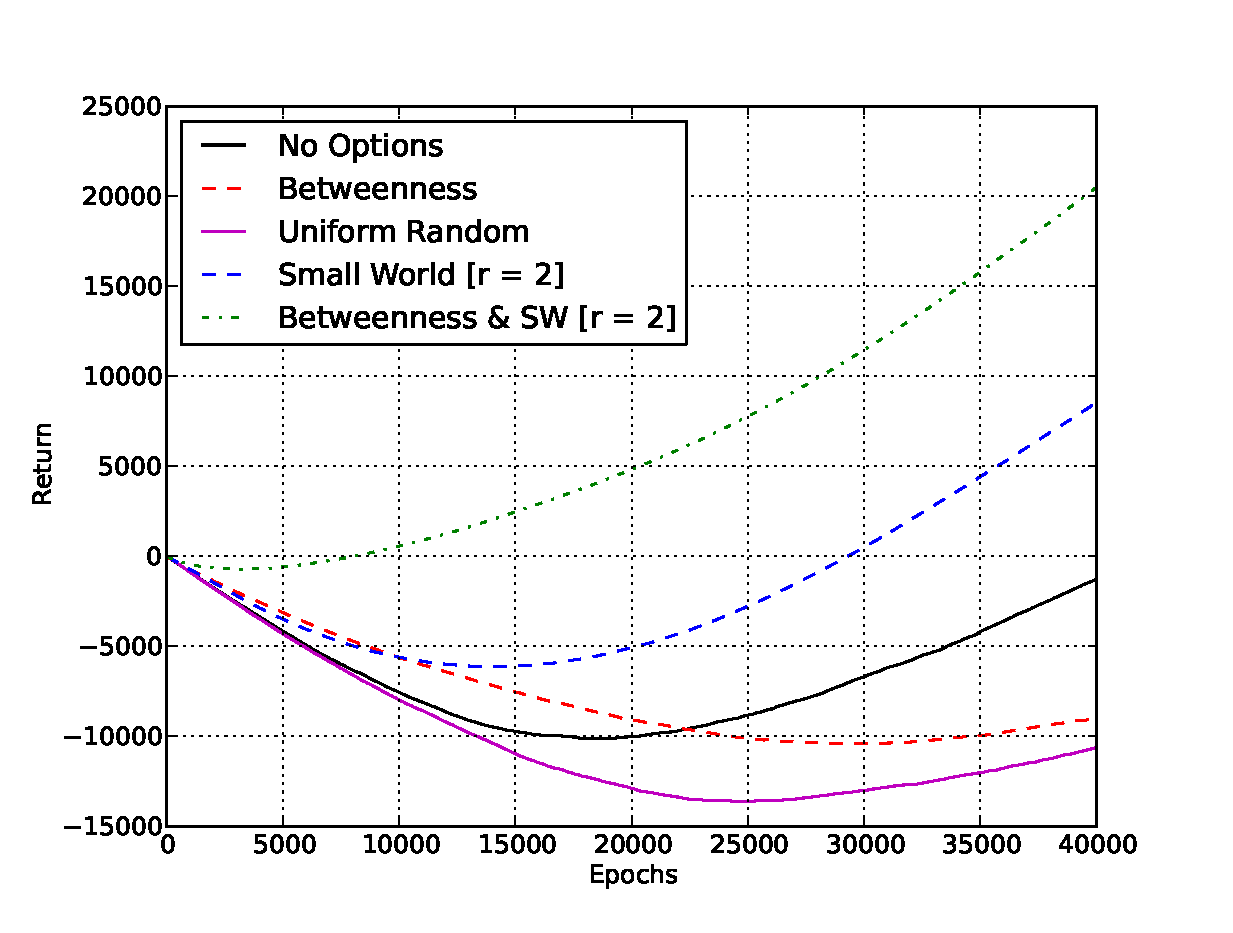
\includegraphics[width=3in]{figures/rooms-200-2}
        \label{fig:rooms-return}
        \caption{Cumulative Return}
    \end{figure}
\end{frame}

\section{Future Work}

\begin{frame}
    \frametitle{}
    \label{frame:future-questions}
    
    \begin{itemize}
        \item How many options do we really need?
        \item Can we make stronger guarantees about the speed of learning in a
            `small-world' (PAC-MDP analysis)?
    \end{itemize}
\end{frame}

\end{document}

% Templates

%\begin{algorithm}
%\caption{C}
%\label{algo:}
%\begin{algorithmic}[1]
%    \STATE 
%    \IF{}
%       \STATE 
%    \ELSE
%       \STATE 
%    \ENDIF
%    \REPEAT
%    \REPEAT
%    \STATE 
%    \FORALL{}
%    \ENDFOR
%    \UNTIL{}
%\end{algorithmic}
%\end{algorithm}

%\begin{IEEEeqnarray*}{rCl}
%\end{IEEEeqnarray*}

%\begin{proof}
%\begin{IEEEeqnarray*}{rCl}
%\end{IEEEeqnarray*}
%\qedhere
%\end{proof}
